Driven by the ability of graphs to represent complex real-world data and capture intricate relationships among entities, research in graph-structured data has been rapidly growing. A core focus of this field is community detection, which involves decomposing a graph into densely connected groups --- revealing the natural structure inherent in the data. Discovering hidden communities in social networks \cite{blekanov2021detection}, analyzing regional retail landscapes \cite{verhetsel2022regional}, studying user relations in Decentralized Online Social Networks (DOSNs) \cite{la2022information}, delineating health care service areas \cite{wang2021network}, uncovering disinformation networks in Telegram \cite{la2021uncovering}, partitioning large graphs for machine learning \cite{bai2024leiden}, studying biological processes \cite{heumos2023best}\ignore{\cite{liu2024sclega, hartman2024peptide, muller2024spatialleiden}}, characterizing polarized information ecosystems\ignore{(climate change conversations)} \cite{uyheng2021mainstream}, developing cyber resilient systems\ignore{/networks by investigating cyber defense techniques} \cite{chernikova2022cyber}, identifying transportation patterns \cite{chen2023deciphering}, identifying attacks in blockchain networks \cite{erfan2023community}, examining restored accounts on Twitter \cite{kapoor2021ll}, exploring the eco-epidemiology of zoonoses \cite{desvars2024one}, analyzing linguistic variation in memes \cite{zhou2023social}, reconstructing multi-step cyber attacks \cite{zang2023attack}, studying twitter communities during the 2022 war in Ukraine \cite{sliwa2024case}, and automated microservice decomposition \cite{cao2022implementation} are all applications of community detection.
% Applications of CD: defending against Distributed Denial of Service (DDoS) \cite{zhao2024ddos}, developing cyber resilient systems/networks by investigating cyber defense techniques \cite{chernikova2022cyber}, 

A challenge in community detection is the absence of prior knowledge about the number and size distribution of communities. To address this, researchers have developed numerous heuristics for finding communities \cite{com-blondel08, com-gregory10}\ignore{\cite{com-raghavan07, com-guimera05, com-derenyi05, com-newman06, com-reichardt06, com-rosvall08, infomap-rosvall09, com-fortunato10, com-kloster14, com-come15, com-ruan15, com-newman16, com-ghoshal19, com-rita20, com-lu20, com-gupta22}}. The quality of identified communities is often measured using fitness metrics such as the modularity score proposed by Newman et al. \cite{com-newman04}. These communities are\ignore{considered} intrinsic when identified based solely on network topology\ignore{, without external attributes}, and they are disjoint when each vertex belongs to only one community \cite{com-gregory10}.
% In summary, no general purpose algorithm will ever serve all applications or data types, because each perspective emphasizes a particular core aspect: a cut-based method provides good separation of balanced groups, a clustering method provides strong cohesiveness of groups with high internal density, stochastic block models provide strong similarity of nodes inside a group in terms of their connectivity profiles, and methods that view communities as dynamical building blocks aim to provide node groups that influence or are influenced by some dynamics in the same way \cite{schaub2017many}.

The Louvain method, proposed by Blondel et al. \cite{com-blondel08}\ignore{from the University of Louvain}, is one of the most popular community detection algorithms \cite{com-lancichinetti09}. This greedy algorithm employs a two-phase approach, consisting of an iterative local-moving phase and an aggregation phase, to iteratively optimize the modularity metric over several passes \cite{com-blondel08}. It has a time complexity of $O(LM)$ (where $M$ is the number of edges in the graph and $L$ is the total number of iterations performed across all passes) and efficiently identifies communities with high modularity.\ignore{What are the popular CD algorithms?}

Despite its popularity, the Louvain method has been observed to produce internally disconnected and poorly connected communities. This problem occurs during the local-moving phase, where important nodes ---\ignore{such as hubs} that serve as bridges within a community --- may be reassigned to another community to which they have stronger connections, breaking the connectivity of their original community. To address these issues, Traag et al. \cite{com-traag19}\ignore{from the University of Leiden} proposed the \textbf{Leiden algorithm}\ignore{ (which is partially based on the smart local move algorithm \cite{waltman2013smart})}, which introduces a refinement phase between the local-moving and aggregation phases. During the refinement phase, vertices can explore and potentially form sub-communities within the communities identified in the local-moving phase --- allowing the algorithm to identify well-connected communities \cite{com-traag19}.
% Note however that neither algorithms, i.e., Louvain and Leiden, can guarantee the convergence to a unique solution every time. One suggestion is to run the programs multiple times to yield a number of results, from which a best solution can be chosen \cite{wang2021network}. A few researchers have observed that the Leiden algorithm is more stable in detecting communities \cite{anuar2021comparison}. Sahu et al. \cite{sahu2024fast} have recently proposed one of the most efficient implementations of the Leiden algorithm.

But many real-world graphs are immense and evolve rapidly over time\ignore{, through the insertion and deletion of edges and vertices}. For efficiency, algorithms are needed that update results without recomputing from scratch, known as \textbf{dynamic algorithms}. Dynamic community detection algorithms also allow one to track the evolution of communities over time, identifying key events like growth, shrinkage, merging, splitting, birth, and death. However, research efforts have focused on detecting communities in dynamic networks using the Louvain algorithm. None of the works have extended these approaches to the Leiden algorithm.
% Parallel algorithms for graph analytics on dynamic graphs are an active area of research. Examples of parallel dynamic algorithms include those for updating centrality scores \cite{cent-shao20, cent-regunta21}, maintaining shortest paths \cite{path-zhang17, path-khanda21}, and dynamic graph coloring \cite{color-yuan17, color-bhattacharya18}.
% Recognizing the temporal dimension's significance, particularly in crisis scenarios, will contribute to a more nuanced understanding of community dynamics \cite{sliwa2024case}.

This paper extends the Naive-dynamic (ND) \cite{com-aynaud10}\ignore{\cite{com-chong13, com-shang14, com-zhuang19}}, Delta-screening (DS) \cite{com-zarayeneh21}, and the recently proposed parallel Dynamic Frontier (DF) approach \cite{sahu2024shared} to the Leiden algorithm.\footnote{\url{https://github.com/puzzlef/leiden-communities-openmp-dynamic}} Our algorithms build on top of GVE-Leiden \cite{sahu2024fast}, one of the most efficient shared-memory implementations of the Static Leiden algorithm.\ignore{Upon receiving a batch update comprising edge deletions and insertions, DF Leiden incrementally identifies and processes an approximate set of affected vertices in an incremental manner. This work represents, to the best of our knowledge, the first endeavor in extending existing dynamic approaches to the Leiden algorithm.}




\subsection{Our Contributions}

We propose the first dynamic algorithms for Leiden, extending dynamic approaches originally developed for Louvain \cite{com-aynaud10, com-zarayeneh21, sahu2024shared} to Leiden. Our contributions are as follows:

\begin{itemize}
  \item Directly applying DF approach \cite{sahu2024shared} to Leiden fails: On a small batch update Leiden's local-moving phase converges quickly. Then refinement phase, divides communities into smaller sub-communities. Terminating at this point (as DF Louvain) results in poor modularity, as these sub-communities require hierarchical aggregation. Consequently, multiple passes of Leiden are needed despite early convergence. This is a key insight.
  \item For selective refinement we track vertices that migrate between communities during local-moving phase, and marking both source and target communities for refinement. Untouched communities are not refined. This reduces processing costs, as refined communities must be processed in subsequent passes.
  \item Refinement begins by initializing each vertex as its own sub-community. These merge into larger sub-communities within their own community bounds. However, this approach applied to a subset of communities can result in internal disconnection. This occurs because a vertex $i$ may not belong to community $C$ with the same ID (i.e., $C = i$), but the initialization places $i$ in an isolated sub-community, while other vertices in community $C$ may not be connected to $i$. As refinement continues, more vertices join $i$ in sub-community $D = i$, yet it remains disconnected from rest of community $C = i$. This insight is illustrated in Figure \ref{fig:subrefine-issue}, and explained in detail in Section \ref{sec:subset-refine-method}.
  \item To resolve this, we propose a subset renumbering procedure where, for each community $C$, the ID of any member vertex $i'$ is selected. This ID is then used to renumber the community membership of all vertices in $C$, update the total edge weight, and set the changed communities flags to the new ID $j$. Afterward, selective refinement can be performed.
  \item We also select communities for refinement based on the batch update (changed communities) - those with edge deletions or insertions within the community. Cross-community edge deletions and insertions are automatically selected when vertices migrate between communities.
  \item Selective refinement causes load imbalance during aggregation phase, as unrefined communities remain large while refined ones are small. To address this, we reduce chunk size for OpenMP parallelization during aggregation, which introduces scheduling overhead but ensures load balancing.
  \item We present novel algorithms\ignore{in this report}, including methods for marking changed-communities and subset-renumbering.
\end{itemize}

\noindent
While reported speedups are modest (DF Leiden is $3.7\times$ faster than Static Leiden for small updates), we believe these insights are crucial for developing more efficient algorithms.




%% - Use --- for a dash.
%% - Use ``camera-ready'' for quotes.
%% - Use {\itshape very} or \textit{very} for italicized text.
%% - Use \verb|acmart| or {\verb|acmart|} for mono-spaced text.
%% - Use \url{https://capitalizemytitle.com/} for URLs.
%% - Use {\bfseries Do not modify this document.} for important boldface details.
%% - Use \ref{fig:name} for referencing.

%% For a block of pre-formatted text: 
% \begin{verbatim}
%   \renewcommand{\shortauthors}{McCartney, et al.}
% \end{verbatim}

%% For a list of items:
% \begin{itemize}
% \item the ``ACM Reference Format'' text on the first page.
% \item the ``rights management'' text on the first page.
% \item the conference information in the page header(s).
% \end{itemize}

%% For a table:
% \begin{table}
%   \caption{Frequency of Special Characters}
%   \label{tab:freq}
%   \begin{tabular}{ccl}
%     \toprule
%     Non-English or Math&Frequency&Comments\\
%     \midrule
%     \O & 1 in 1,000& For Swedish names\\
%     $\pi$ & 1 in 5& Common in math\\
%     \$ & 4 in 5 & Used in business\\
%     $\Psi^2_1$ & 1 in 40,000& Unexplained usage\\
%   \bottomrule
% \end{tabular}
% \end{table}

%% For a full-width table:
% \begin{table*}
%   \caption{Some Typical Commands}
%   \label{tab:commands}
%   \begin{tabular}{ccl}
%     \toprule
%     Command &A Number & Comments\\
%     \midrule
%     \texttt{{\char'134}author} & 100& Author \\
%     \texttt{{\char'134}table}& 300 & For tables\\
%     \texttt{{\char'134}table*}& 400& For wider tables\\
%     \bottomrule
%   \end{tabular}
% \end{table*}


%% For inline math:
% \begin{math}
%   \lim_{n\rightarrow \infty}x=0
% \end{math},

%% For a numbered equation:
% \begin{equation}
%   \lim_{n\rightarrow \infty}x=0
% \end{equation}

%% For an unnumbered equation:
% \begin{displaymath}
%   \sum_{i=0}^{\infty} x + 1
% \end{displaymath}

%% For a figure:
% \begin{figure}[h]
%   \centering
%   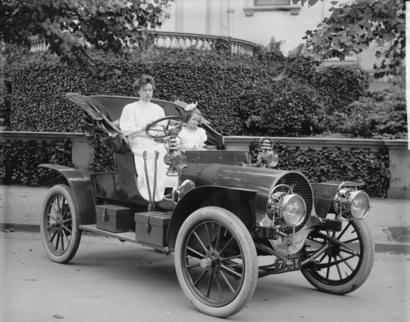
\includegraphics[width=\linewidth]{inc/sample-franklin}
%   \caption{1907 Franklin Model D roadster. Photograph by Harris \&
%     Ewing, Inc. [Public domain], via Wikimedia
%     Commons. (\url{https://goo.gl/VLCRBB}).}
%   \Description{A woman and a girl in white dresses sit in an open car.}
% \end{figure}

%% For a teaser figure.
% \begin{teaserfigure}
%   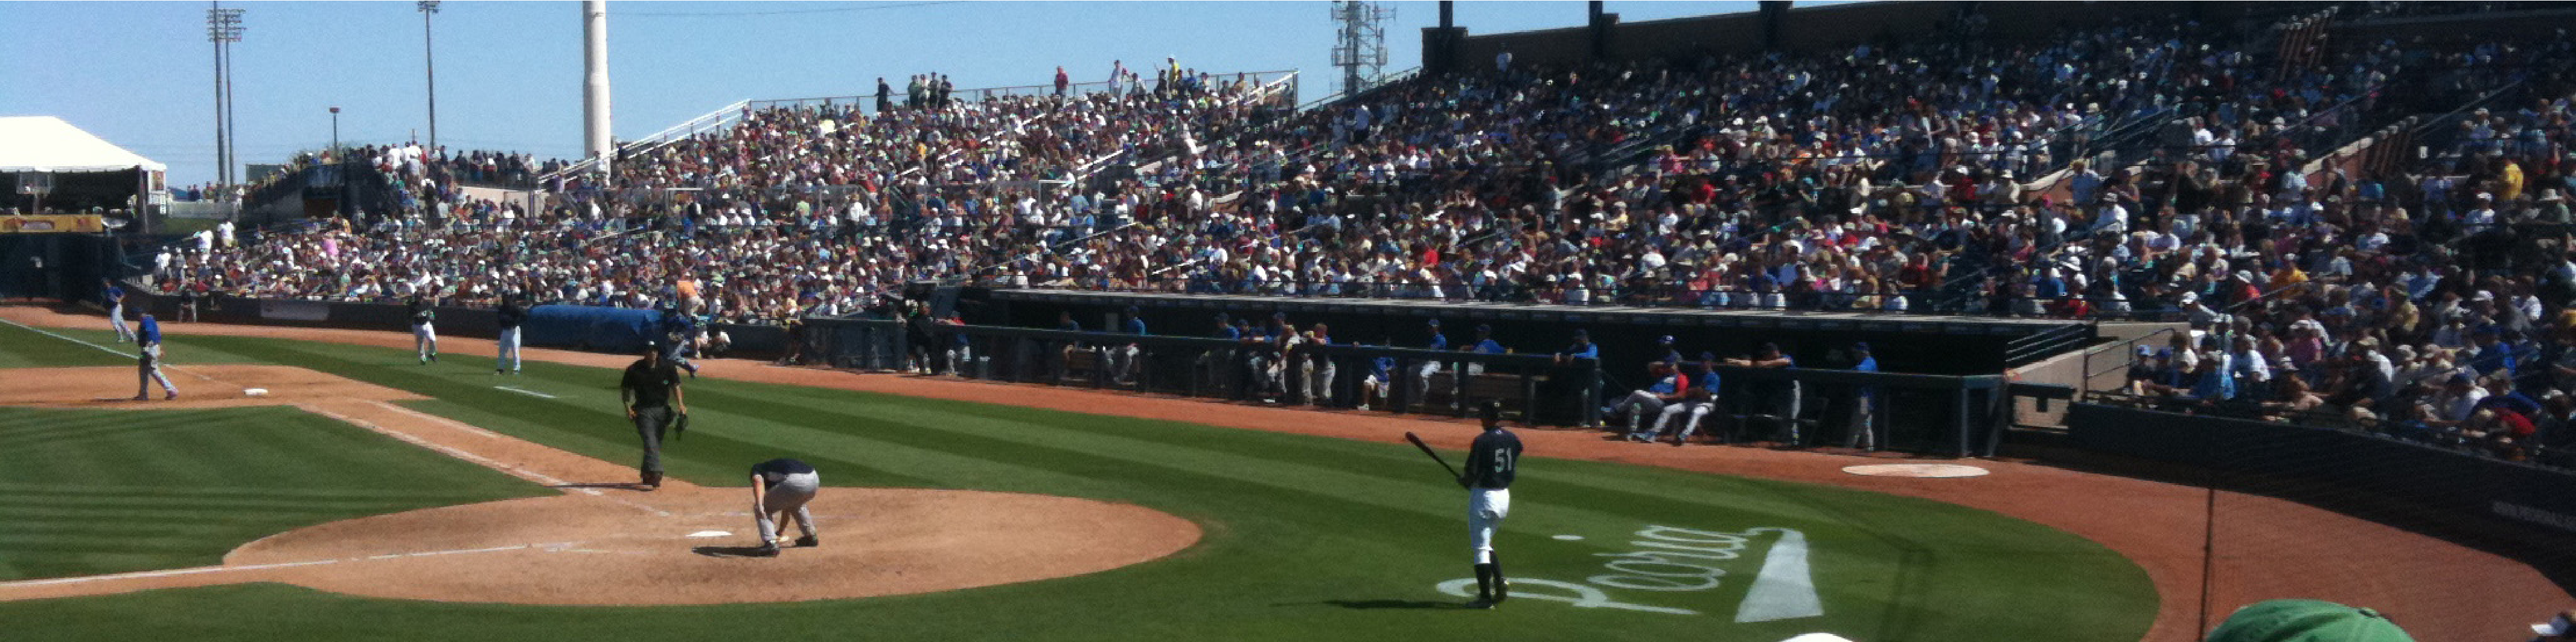
\includegraphics[width=\textwidth]{sampleteaser}
%   \caption{figure caption}
%   \Description{figure description}
% \end{teaserfigure}
